\begin{figure}[!ht]
    % \centering
    \subfloat[Bayes]{
        \label{Bayes}
        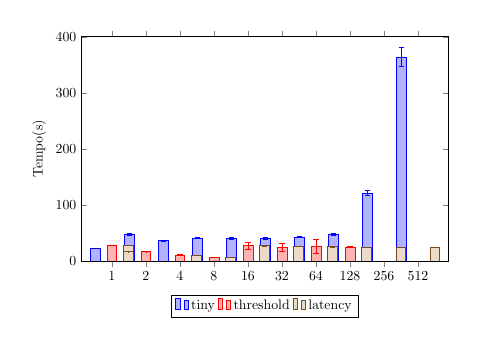
\begin{tikzpicture}[scale=0.5, baseline]
        \begin{axis}[
            width=0.9 \linewidth,
            height=0.6 \linewidth,
            %media de tempo intruder
            ybar=5pt,
            %enlargelimits=0.10,
            legend style={at={(0.5,-0.15)}, anchor=north, legend columns=-1},
            ylabel=Tempo(s),
            symbolic x coords={1, 2, 4, 8, 16, 32, 64, 128, 256, 512},
            xtick=data,
            ymin=0,
            ymax=400,
            bar width=7pt,
            % nodes near coords,
            nodes near coords align={vertical},
        ]
        \addplot+[error bars,y dir=both, y explicit] coordinates {
            (1,22.52)+-(1,0.13) (2,47.52)+-(2,1.02) (4,36.42)+-(4,0.57) (8,41.17)+-(8,1.22) (16,40.32)+-(16,1.21)
            (32,40.14)+-(32,2.42) (64,42.99)+-(64,1.48) (128,47.67)+-(128,2.37) (256,121.10)+-(256,4.24) (512,363.61)+-(512,17.08)}; %orininal
        \addplot+[error bars,y dir=both, y explicit] coordinates {
        (1, 27.79)+-(1,0.14) (2, 16.67)+-(2,0.17) (4, 10.27)+-(4,0.83) (8, 6.64)+-(8,0.30) (16, 27.12)+-(16,6.94) (32, 24.77)+-(32,6.86) (64, 25.93)+-(64,12.29) (128, 24.95)+-(128,0.30) (256, 0.00)+-(256,0.00) (512, 0.00)+-(512,0.00)}; %threshold
        % \addplot+[error bars,y dir=both, y explicit] coordinates {
            % (1, &&)+-(1,**) (2, &&)+-(2,**) (4, &&)+-(4,**) (8, &&)+-(8,**) (16, &&)+-(16,**) (32, &&)+-(32,**) (64, &&)+-(64,**) (128, &&)+-(128,**) (256, &&)+-(256,**) (512, &&)+-(512,**)}; %threshold
        \addplot+[error bars,y dir=both, y explicit] coordinates {
            (1,27.79)+-(1,0.13) (1,16.67)+-(2,0.13) (4,10.27)+-(4,0.13) (8,6.64)+-(8,0.13) (16,27.12)+-(16,0.13)
            (32,26.32)+-(32,0.13) (64,25.30)+-(64,0.13) (128,24.95)+-(128,0.13) (256,24.00)+-(256,0.13) (512,24.00)+-(512,0.13)}; %latency
        \legend {tiny, threshold, latency}
        \end{axis}
        \end{tikzpicture}
    }
    \subfloat[Genome]{
        \label{Genome}
        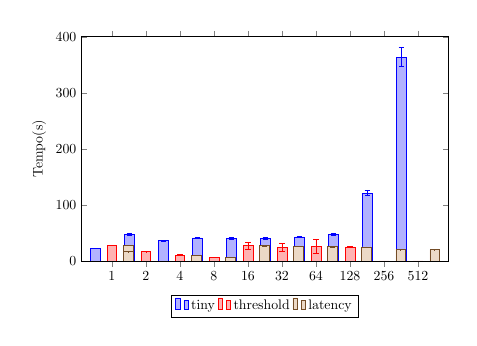
\begin{tikzpicture}[scale=0.5, baseline]
        \begin{axis}[
            width=0.9 \linewidth,
            height=0.6 \linewidth,
            %media de tempo intruder
            ybar=5pt,
            %enlargelimits=0.10,
            legend style={at={(0.5,-0.15)}, anchor=north, legend columns=-1},
            ylabel=Tempo(s),
            symbolic x coords={1, 2, 4, 8, 16, 32, 64, 128, 256, 512},
            xtick=data,
            ymin=0,
            ymax=400,
            bar width=7pt,
            % nodes near coords,
            nodes near coords align={vertical},
        ]
        \addplot+[error bars,y dir=both, y explicit] coordinates {
            (1,22.52)+-(1,0.13) (2,47.52)+-(2,1.02) (4,36.42)+-(4,0.57) (8,41.17)+-(8,1.22) (16,40.32)+-(16,1.21)
            (32,40.14)+-(32,2.42) (64,42.99)+-(64,1.48) (128,47.67)+-(128,2.37) (256,121.10)+-(256,4.24) (512,363.61)+-(512,17.08)}; %orininal
        \addplot+[error bars,y dir=both, y explicit] coordinates {
        (1, 27.79)+-(1,0.14) (2, 16.67)+-(2,0.17) (4, 10.27)+-(4,0.83) (8, 6.64)+-(8,0.30) (16, 27.12)+-(16,6.94) (32, 24.77)+-(32,6.86) (64, 25.93)+-(64,12.29) (128, 24.95)+-(128,0.30) (256, 0.00)+-(256,0.00) (512, 0.00)+-(512,0.00)}; %threshold
        % \addplot+[error bars,y dir=both, y explicit] coordinates {
            % (1, &&)+-(1,**) (2, &&)+-(2,**) (4, &&)+-(4,**) (8, &&)+-(8,**) (16, &&)+-(16,**) (32, &&)+-(32,**) (64, &&)+-(64,**) (128, &&)+-(128,**) (256, &&)+-(256,**) (512, &&)+-(512,**)}; %threshold
        \addplot+[error bars,y dir=both, y explicit] coordinates {
            (1,27.79)+-(1,0.13) (1,16.67)+-(2,0.13) (4,10.27)+-(4,0.13) (8,6.64)+-(8,0.13) (16,27.12)+-(16,0.13)
            (32,26.32)+-(32,0.13) (64,25.30)+-(64,0.13) (128,24.95)+-(128,0.13) (256,20.00)+-(256,0.13) (512,20.00)+-(512,0.13)}; %latency
        % \addplot coordinates {(1,405) (2,365) (4,338) (8,305) (16,263) (32,238) (64,225)}; %mainboard old
        \legend {tiny, threshold, latency}
        \end{axis}
        \end{tikzpicture}
    }
    
    \subfloat[Intruder]{
        \label{Intruder}
        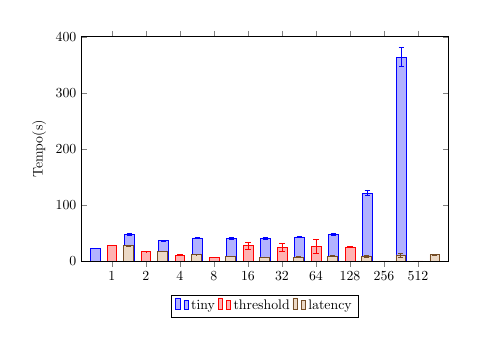
\begin{tikzpicture}[scale=0.5, baseline]
        \begin{axis}[
            width=0.9 \linewidth,
            height=0.6 \linewidth,
            %media de tempo intruder
            ybar=5pt,
            %enlargelimits=0.10,
            legend style={at={(0.5,-0.15)}, anchor=north, legend columns=-1},
            ylabel=Tempo(s),
            symbolic x coords={1, 2, 4, 8, 16, 32, 64, 128, 256, 512},
            xtick=data,
            ymin=0,
            ymax=400,
            bar width=7pt,
            % nodes near coords,
            nodes near coords align={vertical},
        ]
        \addplot+[error bars,y dir=both, y explicit] coordinates {
            (1,22.52)+-(1,0.13) (2,47.52)+-(2,1.02) (4,36.42)+-(4,0.57) (8,41.17)+-(8,1.22) (16,40.32)+-(16,1.21)
            (32,40.14)+-(32,2.42) (64,42.99)+-(64,1.48) (128,47.67)+-(128,2.37) (256,121.10)+-(256,4.24) (512,363.61)+-(512,17.08)}; %orininal
        \addplot+[error bars,y dir=both, y explicit] coordinates {
            (1, 27.79)+-(1,0.14) (2, 16.67)+-(2,0.17) (4, 10.27)+-(4,0.83) (8, 6.64)+-(8,0.30) (16, 27.12)+-(16,6.94) (32, 24.77)+-(32,6.86) (64, 25.93)+-(64,12.29) (128, 24.95)+-(128,0.30) (256, 0.00)+-(256,0.00) (512, 0.00)+-(512,0.00)}; %threshold
        \addplot+[error bars,y dir=both, y explicit] coordinates {
            (1, 27.08)+-(1,0.19) (2, 16.90)+-(2,0.20) (4, 11.40)+-(4,0.14) (8, 8.12)+-(8,0.13) (16, 7.21)+-(16,0.06) (32, 7.29)+-(32,0.11) (64, 8.46)+-(64,1.01) (128, 8.61)+-(128,1.42) (256, 10.73)+-(256,3.40) (512, 11.38)+-(512,0.89)}; %latency
        \legend {tiny, threshold, latency}
        \end{axis}
        \end{tikzpicture}
    }
    \subfloat[Kmeans]{
        \label{Kmeans}
        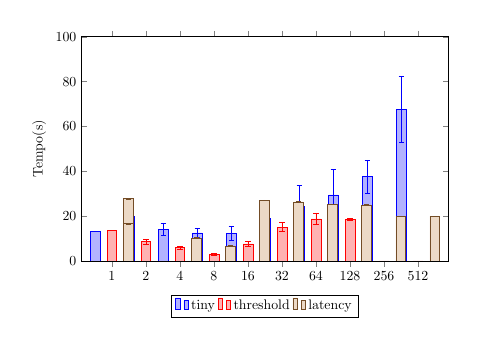
\begin{tikzpicture}[scale=0.5, baseline]
        \begin{axis}[
            width=0.9 \linewidth,
            height=0.6 \linewidth,
            %media de tempo intruder
            ybar=5pt,
            %enlargelimits=0.10,
            legend style={at={(0.5,-0.15)}, anchor=north, legend columns=-1},
            ylabel=Tempo(s),
            symbolic x coords={1, 2, 4, 8, 16, 32, 64, 128, 256, 512},
            xtick=data,
            ymin=0,
            ymax=100,
            bar width=7pt,
            % nodes near coords,
            nodes near coords align={vertical},
        ]
        \addplot+[error bars,y dir=both, y explicit] coordinates {
            (1, 13.31)+-(1,0.04) (2, 19.78)+-(2,2.59) (4, 13.92)+-(4,2.68) (8, 12.52)+-(8,2.06) (16, 12.26)+-(16,2.98) (32, 18.90)+-(32,6.07) (64, 24.16)+-(64,9.41) (128, 29.46)+-(128,11.43) (256, 37.71)+-(256,7.37) (512, 67.63)+-(512,14.92)}; %orininal
        \addplot+[error bars,y dir=both, y explicit] coordinates {
            (1, 13.71)+-(1,0.04) (2, 8.60)+-(2,1.24) (4, 5.95)+-(4,0.77) (8, 3.07)+-(8,0.40) (16, 7.58)+-(16,1.26) (32, 15.06)+-(32,2.00) (64, 18.79)+-(64,2.29) (128, 18.43)+-(128,0.50) (256, 0.00)+-(256,0.00) (512, 0.00)+-(512,0.00)}; %threshold
        \addplot+[error bars,y dir=both, y explicit] coordinates {
            (1,27.79)+-(1,0.13) (1,16.67)+-(2,0.13) (4,10.27)+-(4,0.13) (8,6.64)+-(8,0.13) (16,27.12)+-(16,0.13)
            (32,26.32)+-(32,0.13) (64,25.30)+-(64,0.13) (128,24.95)+-(128,0.13) (256,20.00)+-(256,0.13) (512,20.00)+-(512,0.13)}; %latency
        \legend {tiny, threshold, latency}
        \end{axis}
        \end{tikzpicture}
    }

    \subfloat[Labyrinth]{
        \label{Labyrinth}
        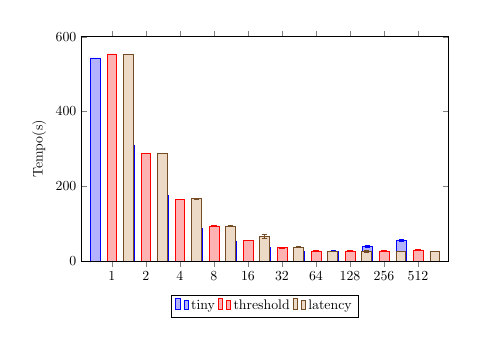
\begin{tikzpicture}[scale=0.5, baseline]
        \begin{axis}[
            width=0.9 \linewidth,
            height=0.6 \linewidth,
            %media de tempo intruder
            ybar=5pt,
            %enlargelimits=0.10,
            legend style={at={(0.5,-0.15)}, anchor=north, legend columns=-1},
            ylabel=Tempo(s),
            symbolic x coords={1, 2, 4, 8, 16, 32, 64, 128, 256, 512},
            xtick=data,
            ymin=0,
            ymax=600,
            bar width=7pt,
            % nodes near coords,
            nodes near coords align={vertical},
        ]
        \addplot+[error bars,y dir=both, y explicit] coordinates {
            (1, 543.18)+-(1,0.30) (2, 308.18)+-(2,4.18) (4, 174.91)+-(4,4.30) (8, 86.27)+-(8,1.05) (16, 51.52)+-(16,1.12)
            (32, 36.01)+-(32,1.19) (64, 26.37)+-(64,1.12) (128, 26.41)+-(128,1.34) (256, 39.65)+-(256,2.30) (512, 55.76)+-(512,2.54)}; %orininal
        \addplot+[error bars,y dir=both, y explicit] coordinates {
            (1, 553.85)+-(1,0.17) (2, 287.47)+-(2,0.51) (4, 165.29)+-(4,0.86) (8, 93.59)+-(8,0.93) (16, 54.92)+-(16,0.82) (32, 35.24)+-(32,0.84) (64, 26.63)+-(64,1.47) (128, 26.36)+-(128,1.37) (256, 26.86)+-(256,1.49) (512, 29.29)+-(512,1.90)}; %threshold
        \addplot+[error bars,y dir=both, y explicit] coordinates {
            (1, 553.60)+-(1,0.40) (2, 287.68)+-(2,0.34) (4, 166.47)+-(4,1.20) (8, 93.88)+-(8,1.15) (16, 65.32)+-(16,5.74) (32, 36.78)+-(32,1.08) (64, 25.43)+-(64,0.91) (128, 25.32)+-(128,1.91) (256, 25.59)+-(256,1.14) (512, 26.01)+-(512,0.64)}; %latency
        \legend {tiny, threshold, latency}
        \end{axis}
        \end{tikzpicture}
    }
    \subfloat[SSCA2]{
        \label{SSCA2}
        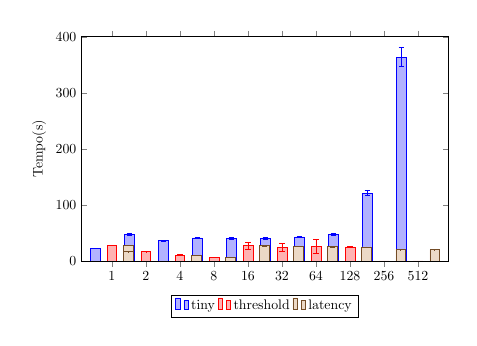
\begin{tikzpicture}[scale=0.5, baseline]
        \begin{axis}[
            width=0.9 \linewidth,
            height=0.6 \linewidth,
            %media de tempo intruder
            ybar=5pt,
            %enlargelimits=0.10,
            legend style={at={(0.5,-0.15)}, anchor=north, legend columns=-1},
            ylabel=Tempo(s),
            symbolic x coords={1, 2, 4, 8, 16, 32, 64, 128, 256, 512},
            xtick=data,
            ymin=0,
            ymax=400,
            bar width=7pt,
            % nodes near coords,
            nodes near coords align={vertical},
        ]
        \addplot+[error bars,y dir=both, y explicit] coordinates {
            (1,22.52)+-(1,0.13) (2,47.52)+-(2,1.02) (4,36.42)+-(4,0.57) (8,41.17)+-(8,1.22) (16,40.32)+-(16,1.21)
            (32,40.14)+-(32,2.42) (64,42.99)+-(64,1.48) (128,47.67)+-(128,2.37) (256,121.10)+-(256,4.24) (512,363.61)+-(512,17.08)}; %orininal
        \addplot+[error bars,y dir=both, y explicit] coordinates {
            (1, 27.79)+-(1,0.14) (2, 16.67)+-(2,0.17) (4, 10.27)+-(4,0.83) (8, 6.64)+-(8,0.30) (16, 27.12)+-(16,6.94) (32, 24.77)+-(32,6.86) (64, 25.93)+-(64,12.29) (128, 24.95)+-(128,0.30) (256, 0.00)+-(256,0.00) (512, 0.00)+-(512,0.00)}; %threshold
        % \addplot+[error bars,y dir=both, y explicit] coordinates {
            % (1, &&)+-(1,**) (2, &&)+-(2,**) (4, &&)+-(4,**) (8, &&)+-(8,**) (16, &&)+-(16,**) (32, &&)+-(32,**) (64, &&)+-(64,**) (128, &&)+-(128,**) (256, &&)+-(256,**) (512, &&)+-(512,**)}; %threshold
        \addplot+[error bars,y dir=both, y explicit] coordinates {
            (1,27.79)+-(1,0.13) (1,16.67)+-(2,0.13) (4,10.27)+-(4,0.13) (8,6.64)+-(8,0.13) (16,27.12)+-(16,0.13)
            (32,26.32)+-(32,0.13) (64,25.30)+-(64,0.13) (128,24.95)+-(128,0.13) (256,20.00)+-(256,0.13) (512,20.00)+-(512,0.13)}; %latency
        % \addplot coordinates {(1,405) (2,365) (4,338) (8,305) (16,263) (32,238) (64,225)}; %mainboard old
        \legend {tiny, threshold, latency}
        \end{axis}
        \end{tikzpicture}
    }

    \subfloat[Vacation]{
        \label{Vacation}
        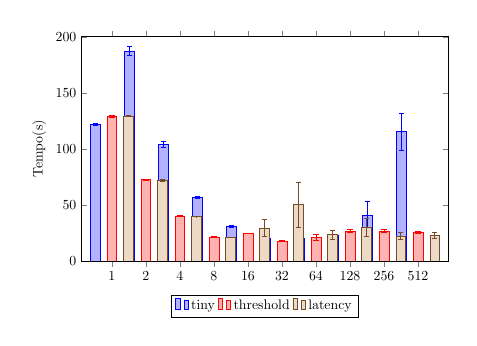
\begin{tikzpicture}[scale=0.5, baseline]
        \begin{axis}[
            width=0.9 \linewidth,
            height=0.6 \linewidth,
            %media de tempo intruder
            ybar=5pt,
            %enlargelimits=0.10,
            legend style={at={(0.5,-0.15)}, anchor=north, legend columns=-1},
            ylabel=Tempo(s),
            symbolic x coords={1, 2, 4, 8, 16, 32, 64, 128, 256, 512},
            xtick=data,
            ymin=0,
            ymax=200,
            bar width=7pt,
            % nodes near coords,
            nodes near coords align={vertical},
        ]
        \addplot+[error bars,y dir=both, y explicit] coordinates {
            (1, 122.10)+-(1,0.80) (2, 187.32)+-(2,4.17) (4, 103.98)+-(4,2.34) (8, 56.82)+-(8,1.03) (16, 30.99)+-(16,1.17)
            (32, 19.91)+-(32,0.76) (64, 19.86)+-(64,4.36) (128, 22.96)+-(128,0.70) (256, 40.62)+-(256,12.24) (512, 115.22)+-(512,16.30)};%original
        \addplot+[error bars,y dir=both, y explicit] coordinates {
            (1, 129.22)+-(1,1.06) (2, 72.49)+-(2,0.37) (4, 40.07)+-(4,0.28) (8, 21.51)+-(8,0.18) (16, 24.69)+-(16,0.20) (32, 17.61)+-(32,0.48) (64, 20.84)+-(64,2.57) (128, 26.60)+-(128,1.50) (256, 26.84)+-(256,1.64) (512, 25.82)+-(512,1.05)}; %threshold
        \addplot+[error bars,y dir=both, y explicit] coordinates {
            (1, 129.47)+-(1,0.79) (2, 72.00)+-(2,0.52) (4, 39.61)+-(4,0.21) (8, 21.20)+-(8,0.13) (16, 29.52)+-(16,7.38) (32, 50.24)+-(32,20.35) (64, 23.66)+-(64,4.03) (128, 30.27)+-(128,7.94) (256, 22.20)+-(256,3.14) (512, 22.86)+-(512,2.40)}; %latency
        \legend {tiny, threshold, latency}
        \end{axis}
        \end{tikzpicture}
    }
    \subfloat[Yada]{
        \label{Yada}
        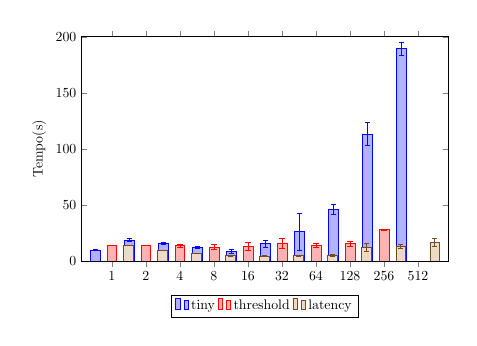
\begin{tikzpicture}[scale=0.5, baseline]
        \begin{axis}[
            width=0.9 \linewidth,
            height=0.6 \linewidth,
            %media de tempo intruder
            ybar=5pt,
            %enlargelimits=0.10,
            legend style={at={(0.5,-0.15)}, anchor=north, legend columns=-1},
            ylabel=Tempo(s),
            symbolic x coords={1, 2, 4, 8, 16, 32, 64, 128, 256, 512},
            xtick=data,
            ymin=0,
            ymax=200,
            bar width=7pt,
            % nodes near coords,
            nodes near coords align={vertical},
        ]
        \addplot+[error bars,y dir=both, y explicit] coordinates {
            (1, 9.91)+-(1,0.05) (2, 18.83)+-(2,0.94) (4, 15.66)+-(4,1.17) (8, 12.14)+-(8,1.24) (16, 8.61)+-(16,1.66)
            (32, 15.32)+-(32,3.18) (64, 26.12)+-(64,16.23) (128, 46.30)+-(128,4.30) (256, 113.08)+-(256,10.17) (512, 189.68)+-(512,5.81)}; %orininal
        \addplot+[error bars,y dir=both, y explicit] coordinates {
            (1, 14.13)+-(1,0.08) (2, 14.18)+-(2,0.14) (4, 13.65)+-(4,1.53) (8, 12.30)+-(8,2.15) (16, 13.01)+-(16,3.46) (32, 15.69)+-(32,4.47) (64, 14.00)+-(64,2.04) (128, 15.66)+-(128,2.22) (256, 27.88)+-(256,0.21) (512, 0.00)+-(512,0.00)}; %threshold
        \addplot+[error bars,y dir=both, y explicit] coordinates {
            (1, 14.08)+-(1,0.10) (2, 9.88)+-(2,0.04) (4, 7.20)+-(4,0.05) (8, 4.69)+-(8,0.35) (16, 4.57)+-(16,0.54) (32, 4.67)+-(32,0.42) (64, 5.38)+-(64,0.92) (128, 12.36)+-(128,3.68) (256, 13.03)+-(256,1.89) (512, 16.39)+-(512,3.62)}; %latency         
        \legend {tiny, threshold, latency}
        \end{axis}
        \end{tikzpicture}
    }
    
    \caption{Tempo de execução (s) em NUMA variando o número de \emph{threads}.}
    \label{temp}

\end{figure}
% (1, &&)+-(1,**) (2, &&)+-(2,**) (4, &&)+-(4,**) (8, &&)+-(8,**) (16, &&)+-(16,**) (32, &&)+-(32,**) (64, &&)+-(64,**) (128, &&)+-(128,**) (256, &&)+-(256,**) (512, &&)+-(512,**)}; %threshold
